\documentclass[final]{beamer}

% ====================
% Packages
% ====================
\usepackage[T1]{fontenc}
\usepackage{lmodern}
\usepackage[size=custom,width=120,height=72,scale=1.0]{beamerposter}
\usetheme{gemini}
\usecolortheme{cam}
\usepackage{graphicx}
\usepackage{svg}
\usepackage{booktabs}
\usepackage[numbers]{natbib}
\usepackage{tikz}
\usepackage{pgfplots}
\pgfplotsset{compat=1.14}
\usepackage{anyfontsize}

% ====================
% Lengths for Columns
% ====================
% If you have N columns, choose \sepwidth and \colwidth such that
% (N+1)*\sepwidth + N*\colwidth = \paperwidth
\newlength{\sepwidth}
\newlength{\colwidth}
\setlength{\sepwidth}{0.025\paperwidth}
\setlength{\colwidth}{0.3\paperwidth}
\newcommand{\separatorcolumn}{\begin{column}{\sepwidth}\end{column}}

% ====================
% Title and Author
% ====================
\title{\centering Analysis of Leakage Suppression in Transmon Qubits \\ Under Different DRAG Drives}
\author{Uday Mathur \inst{1} \and Sandeep Joshi \inst{2} \and Prashant Shukla \inst{2}}
\institute[shortinst]{
    \inst{1} Dept. of Physics, Indian Institute of Technology (BHU), Varanasi, India
    \samelineand
    \inst{2} Nuclear Physics Division, Bhabha Atomic Research Centre, Mumbai, India
}

% ====================
% Footer (optional)
% ====================
\footercontent{
    \href{https://www.example.com}{uday.mathur.cd.phy22@itbhu.ac.in}
    \hfill IWQT-2025
    \hfill \href{mailto:alyssa.p.hacker@example.com}{pshuklabarc@gmail.com}
}

% ====================
% Logos (optional)
% ====================
\logoleft{
\includegraphics[height=7cm]{Logos/BARC_logo.png}}
\logoright{
\includegraphics[height=7cm]{Logos/IWQT_logo.jpg}}

% ====================
% Document Start
% ====================
\begin{document}

% Optional header tweak if needed
%\addtobeamertemplate{headline}{}{}

\begin{frame}[t]
    \begin{columns}[t]

        % --- Column 1 ---
        \separatorcolumn
        \begin{column}{\colwidth}

            % Research Purpose Block
            \begin{block}{Research Purpose}
                Currently, large-scale superconducting quantum processors rely on Transmon qubits, which suffer from low anharmonicity and frequency crowding, typically in the range \(|\alpha/2\pi| \in [150, 300]\,\text{MHz}\). This leads to spectral overlap of control pulses with higher-level transitions, such as \(|1\rangle \leftrightarrow |2\rangle\), causing leakage errors. To mitigate this, we study \textbf{pulse-shaping techniques} that suppress leakage while maintaining fast and high-fidelity single-qubit gates.
            \end{block}

            % What We Did Block
            \begin{block}{What we did}
                We performed a comparative simulation of DRAG, fifth-order DRAG, FAST DRAG, and HD DRAG pulses using a three-level Transmon model to implement an X-gate. In the rotating frame at drive frequency \(f_d\), the Hamiltonian is:
                \[
                H_R = \sum_j \left( \delta_j |j\rangle\langle j| + \frac{I(t)}{2}\sigma_x^{j-1,j} + \frac{Q(t)}{2}\sigma_y^{j-1,j} \right),
                \]
                with leakage arising from coupling to higher excited states and the quadrature envelope defined as:
                \[
                Q(t) = -\beta\, \frac{\dot{I}(t)}{\alpha},
                \]
                following the DRAG scheme.

                We analyzed the average gate infidelity for Gaussian pulses across different DRAG coefficients (\(\beta\)) and compared it with the fifth-order DRAG expansion incorporating time-dependent detuning as illustrated in Figure 1.

                FAST and HD pulses were evaluated by examining leakage suppression around the anharmonic frequency (\(\alpha/2\pi = -212\,\text{MHz}\)) in Figure 2(a).

                In Figure 3, we studied the sensitivity of average gate fidelity to coherent errors—leakage and phase—using the leakage rate \(\mathcal{L}_1\) and seepage rate \(\mathcal{L}_2\), defined as:
                \[
                \mathcal{L}_1 = \frac{1}{d_1} \mathrm{Tr}[I_2 U_r I_1 U_r^\dagger], \quad
                \mathcal{L}_2 = 1 - \frac{1}{d_2} \mathrm{Tr}[I_2 U_r I_2 U_r^\dagger].
                \]

                \begin{figure}
                    \centering
                    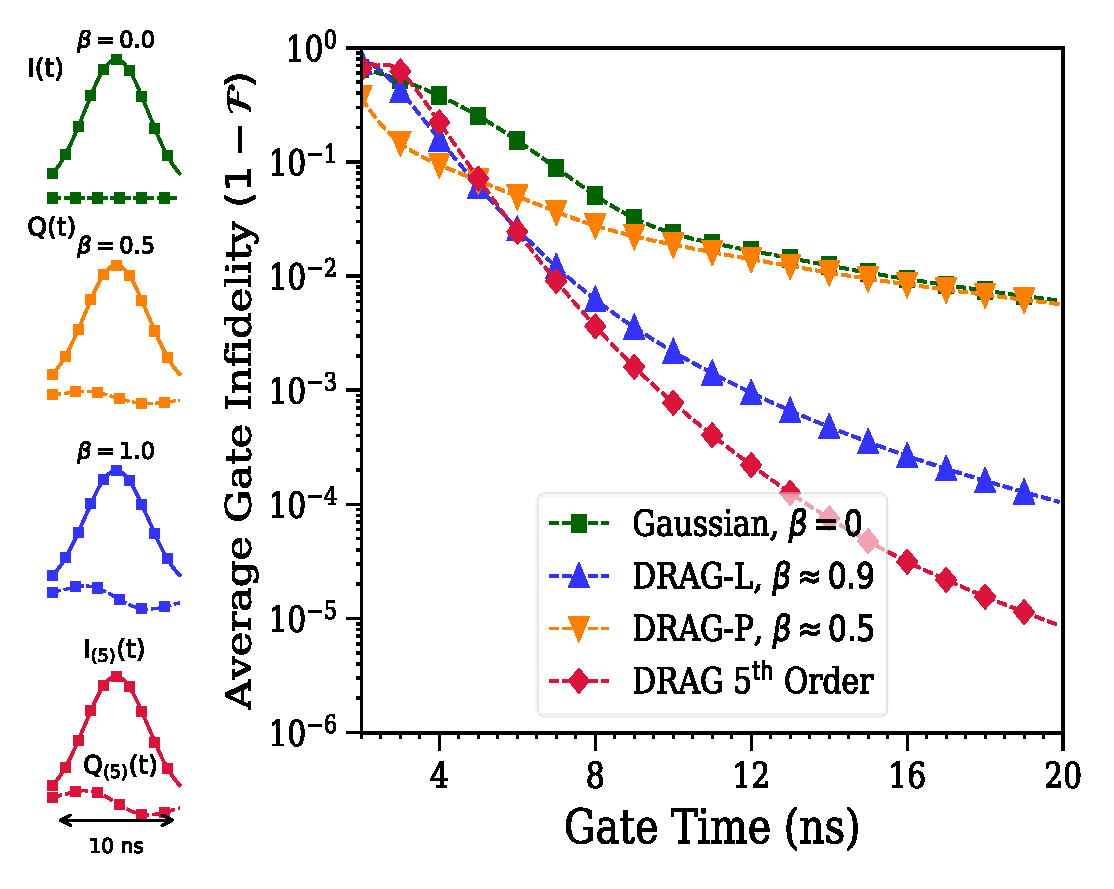
\includegraphics[width=0.6\linewidth]{Images_pdfs/IWQT_gauss_pulse-fidelity.pdf}
                    \caption{Pulse envelopes \(I(t)\) and \(Q(t)\) for different DRAG parameters \(\beta\), with \(\beta=0\) corresponding to a Gaussian pulse, \(\beta=0.5\) to the DRAG-P scheme (phase correction), \(\beta=0.1\) to the DRAG-L (leakage suppression), with 5th-order DRAG correction \(I_5(t)\). (Right) Average gate infidelity \((1-\mathcal{F})\) versus gate time \(t_g\).}
                \end{figure}
            \end{block}

        \end{column}

        % --- Column 2 ---
        \separatorcolumn
        \begin{column}{\colwidth}

            % Simulation and Analysis Block
            \begin{block}{Simulation and Analysis}
                \begin{figure}
                    \centering
                    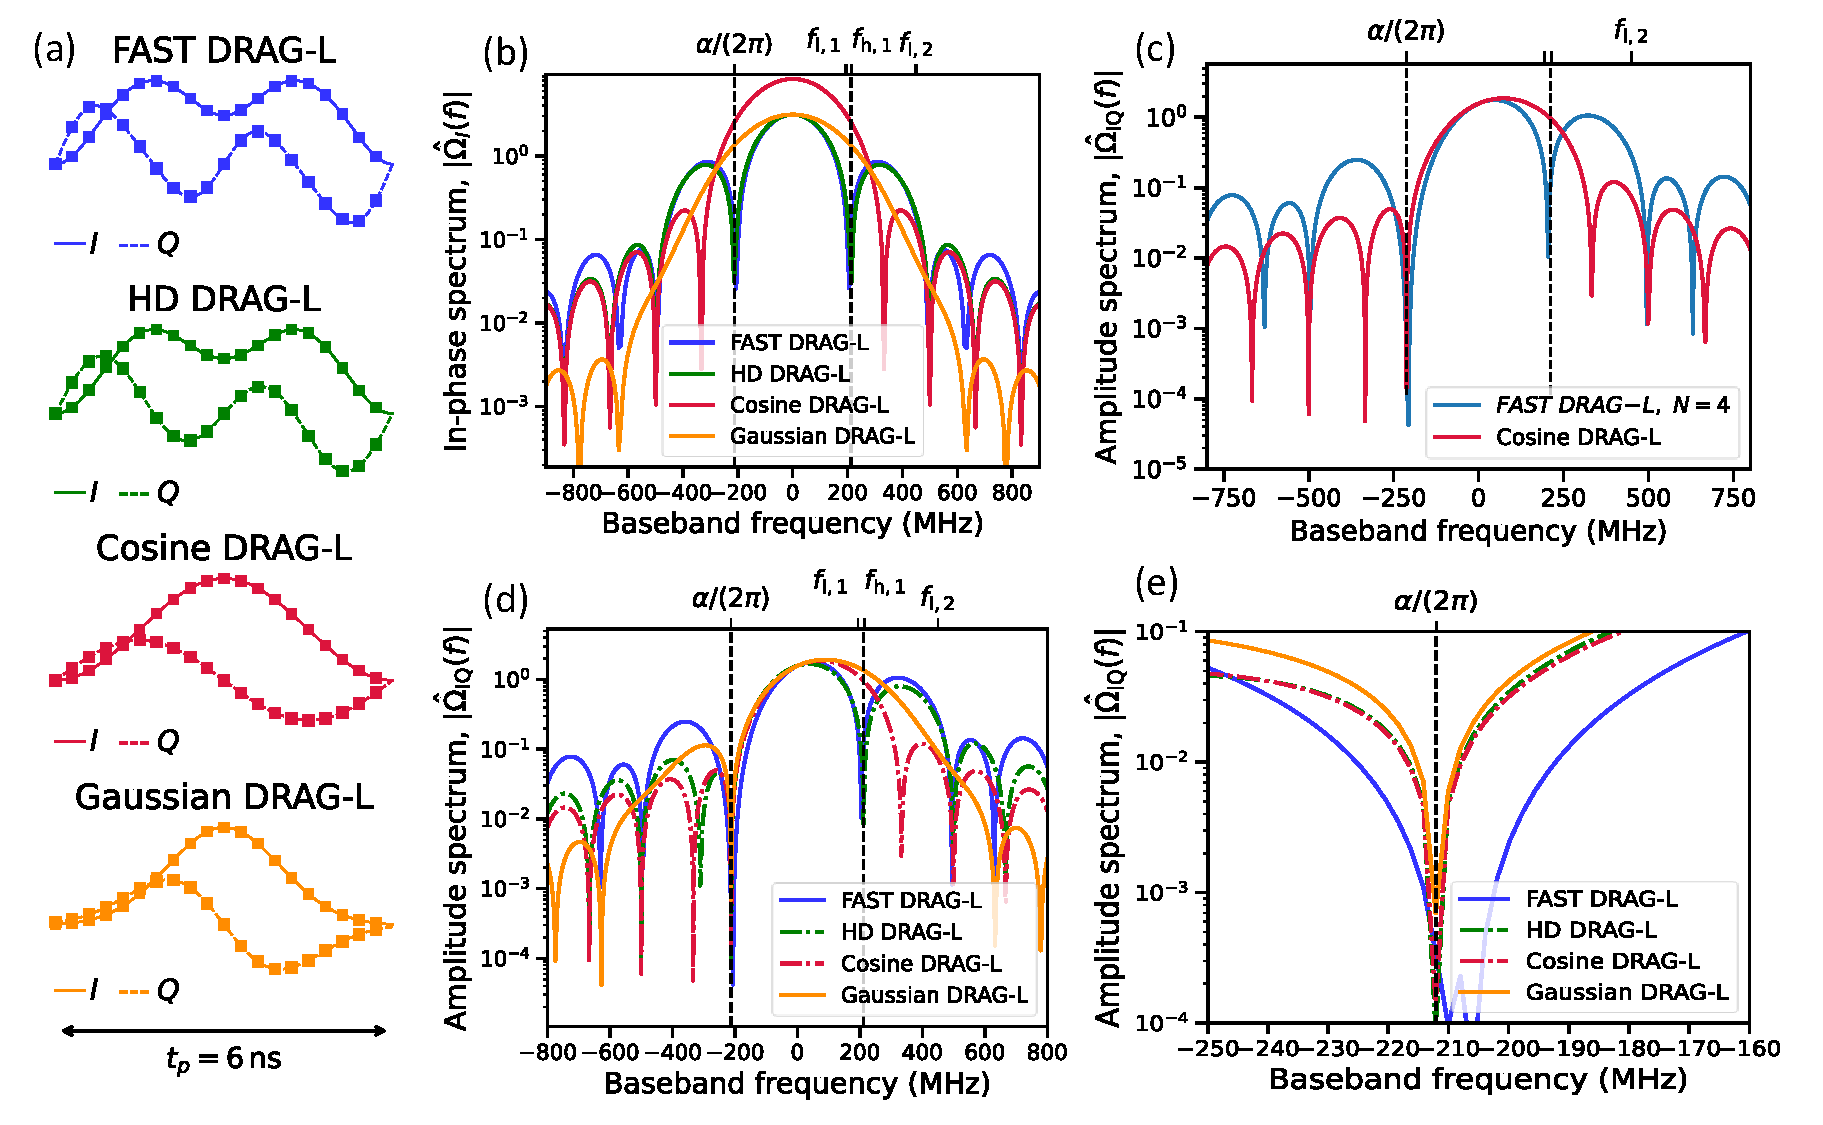
\includegraphics[width=0.9\linewidth]{Images_pdfs/IWQT-FAST&HD-leakage-spectrum.pdf}
                    \caption{
                        (a) In-phase (\textit{I}, solid) and quadrature (\textit{Q}, dashed) components for FAST DRAG-L (dark blue), HD DRAG-L (dark green), raised-cosine DRAG (red), and Gaussian DRAG (dark orange) with \(\beta \approx 1.0\).
                        (b) Amplitude spectrum \(\lvert \hat\Omega_I(f) \rvert\) of \(I(t)\).
                        (c) Leakage spectrum for FAST DRAG-L and raised-cosine.
                        (d) Amplitude spectrum \(\lvert \hat\Omega_{IQ}(f) \rvert\) of \(\Omega_{IQ}(t)\) showing suppression at the qubit anharmonicity \(\alpha/(2\pi)\) (dashed line).
                        (e) Bandwidth of suppression at anharmonicity \(\alpha/2\pi\) showing maximum bandwidth of FAST DRAG-L.
                    }
                \end{figure}
            \end{block}

            % Example Block for FAST and HD Pulses
            \begin{exampleblock}{Fourier ansatz spectrum tuning (FAST) and Higher Derivative (HD) Pulses}
                FAST shapes the in-phase envelope to suppress spectral components near the anharmonic frequency, while DRAG generates the quadrature component to further minimize leakage, thus giving FAST DRAG.

                \[
                \Omega_I(t) = A_0 + \sum_{n=1}^{N} A_n \cos\left(\frac{n\pi t}{T}\right),
                \]

                \heading{FAST DRAG -- Spectral Optimization}

                The FAST DRAG optimization aims to minimize the spectral amplitude around the anharmonic frequency:
                \[
                \min_{\{A_n\}} \int_{f_{l,1}}^{f_{h,1}} \left| \hat{\Omega}_I(f) \right|^{2} \, df,
                \]

                \heading{HD DRAG -- Higher Derivatives}

                The \textbf{HD DRAG} method includes derivatives up to the second order in \(I(t)\) and up to the third order in \(Q(t)\):
                \[
                I(t) = A \left[ \Omega_I(t) + \beta_2 \ddot{\Omega}_I(t) \right], \quad
                Q(t) = -\frac{A \beta}{\alpha} \left[ \dot{\Omega}_I(t) + \beta_2 \dddot{\Omega}_I(t) \right].
                \]
            \end{exampleblock}

        \end{column}

        % --- Column 3 ---
        \separatorcolumn
        \begin{column}{\colwidth}

            % Results and Observations Block
            \begin{alertblock}{What We Saw}
                Advanced pulse-shaping techniques—FAST DRAG and HD DRAG—effectively suppress leakage and improve gate fidelity in weakly anharmonic superconducting qubits.

                While HD DRAG offers a straightforward approach with fewer calibration parameters, FAST DRAG delivers greater flexibility in spectral control and bandwidth tuning, making it especially advantageous for complex multi-level systems.

                \begin{itemize}
                    \item \textbf{Phase Error Sensitivity:} Gate fidelity is more significantly impacted by phase accumulation before and after the pulse than by leakage errors, as demonstrated in Figure 3.
                    \item \textbf{Enhanced Spectral Suppression:} FAST DRAG pulses provide stronger and broader suppression of spectral components near the qubit anharmonic frequency compared to traditional raised-cosine and Gaussian envelopes, as shown in Figure 2(c).
                    \item \textbf{Optimized Bandwidth Control:} The FAST method enables precise pulse spectrum shaping, allowing fine control over bandwidth and amplitude without sacrificing gate fidelity, as illustrated in Figure 2(e).
                \end{itemize}

                \textbf{Takeaway:} Gate fidelity is predominantly limited by phase errors. FAST DRAG offers flexible, high-fidelity control, whereas HD DRAG serves as a simpler, low-calibration alternative.
            \end{alertblock}

            % Figure 3 Block
            \begin{figure}
                \centering
                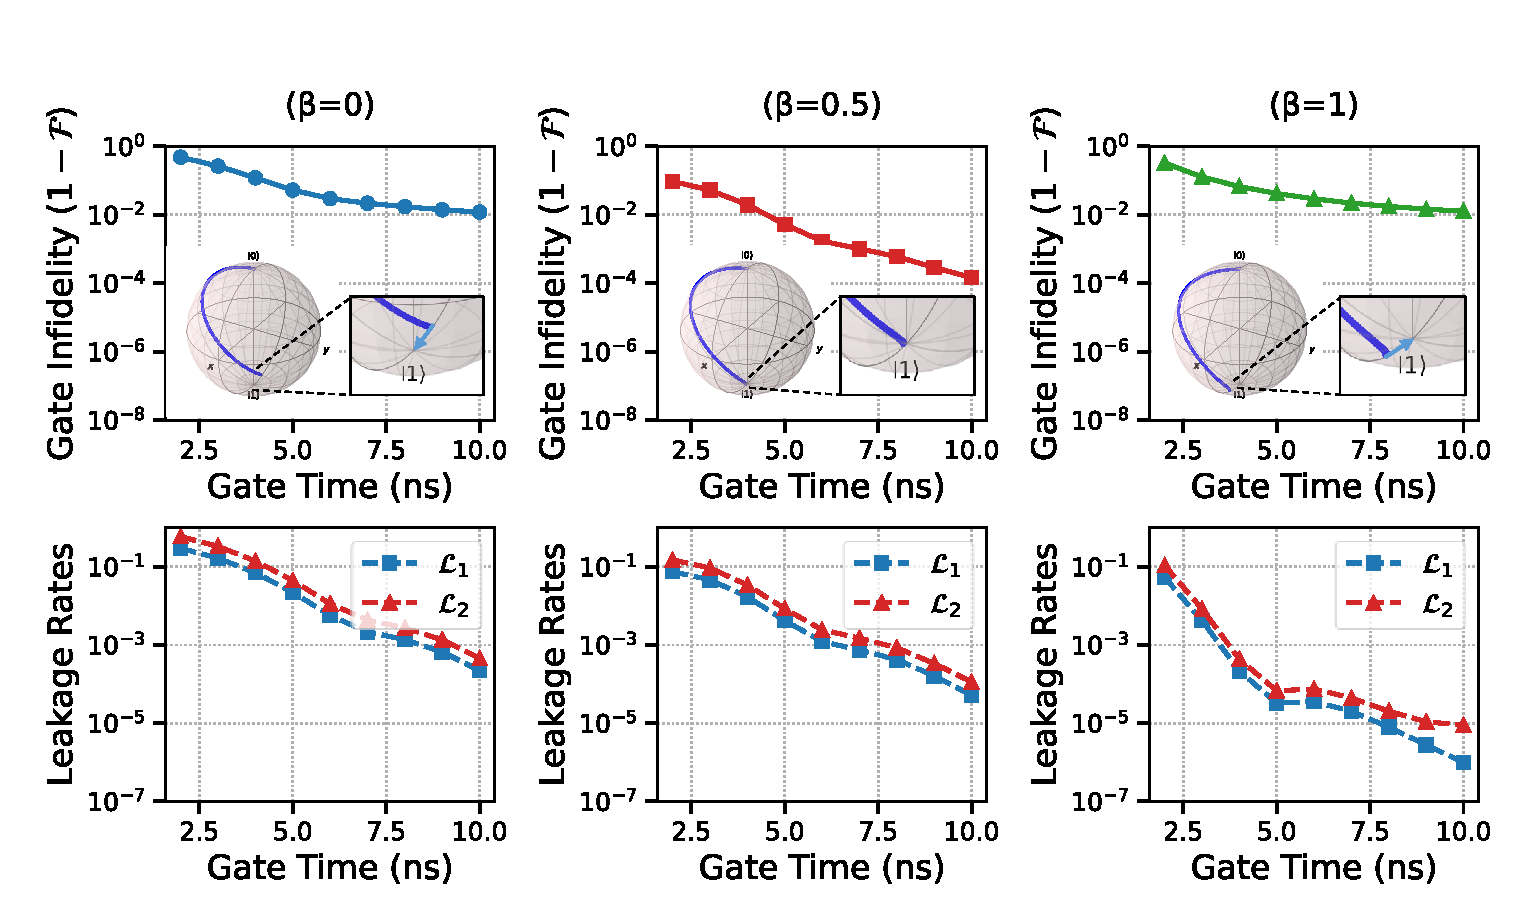
\includegraphics[width=\linewidth]{Images_pdfs/IWQT-Gaussian_fidelity-L1andL2.pdf}
                \caption{
                    Gate performance for Gaussian (left) and DRAG pulses with \(\beta=0.5\) (middle) and \(\beta=1.0\) (right).

                    \textit{Upper row:} Average gate infidelity versus gate time with Bloch sphere trajectories showing qubit evolution. The \(\beta=0.5\) case (DRAG-P) provides phase correction with limited leakage suppression, while \(\beta=1.0\) (DRAG-L) yields stronger leakage suppression.
                    \textit{Lower row:} Leakage \(\mathcal{L}_1\) and seepage \(\mathcal{L}_2\) as functions of gate time, both decreasing with longer gates, with \(\beta=1.0\) giving superior suppression compared to \(\beta=0.5\).
                }
            \end{figure}

            % References Block
            \nocite{*}
            \begin{block}{References}
                \bibliographystyle{plainnat}
                \bibliography{poster}
            \end{block}
        \end{column}

        \separatorcolumn
    \end{columns}
\end{frame}

\end{document}
